%================================================================%
%======  Modelo de Monografia ( UFOP - DECOM) ===================%
% Proposta de texto em conformidade com normas da ABNT ----------%
% implementadas pelo projeto abntex2, que pode ser acessado pela %
% página  http://abntex2.googlecode.com/  -----------------------%
%================================================================%
\documentclass[12pt, % tamanho da fonte
   %openright,	     % capítulos começam em pág ímpar
	oneside,		  % twoside para impressão em frente e verso.  
	a4paper,			% tamanho do papel. 
	english,			% Idioma adicional para hifenizaç
    brazil,				% Idioma principal 
    sumario=tradicional % Comente para o sumário ser conforme a opção padrão recomendada pela ABNT NBR 6027:2012.
	]{abntex2}
	
%------------------------------------------------------------
%------------    Estrutura do texto   -----------------------         

% Pacotes Básicos:
\usepackage{lmodern}			% Fonte Latin Modern			
\usepackage[T1]{fontenc}		% Seleção de codigos de fonte.
\usepackage[utf8]{inputenc}		% Codificacao do documento (conversão automática dos acentos)
\usepackage{lastpage}		    % Usado pela Ficha catalográfica
\usepackage{indentfirst}		% Indenta o primeiro parágrafo de cada seção.
\usepackage{color}				% Controle das cores
\usepackage{graphicx}			% Inclusão de gráficos
\usepackage{tabularx}
\usepackage{microtype} 		  	% Melhorias da justificação

% Pacotes Extras:
\usepackage{amsmath,amsthm}     % Símbolos Matemáticos
\usepackage[portuguese, ruled, linesnumbered,commentsnumbered, algo2e, vlined, lined, boxed, algochapter]{algorithm2e} % Algoritmos 
\usepackage{hyperref}      % Criação de links.

% Escolha da formatação das referências Bibliográficass: 
\usepackage[alf]{abntex2cite}	% Citações padrão ABNT  (AUTOR, ANO)
\usepackage{etoolbox}
%\usepackage[num]{abntex2cite}  % Citações numéricas (1)
%\citebrackets[] % Usar este comando para a citação numérica aparecer com [].

% Numeração das Figuras e Tabelas
\counterwithin{figure}{chapter}
\counterwithin{table}{chapter}

% Defininção de Cores:
\definecolor{blue}{RGB}{25,25,112}
\makeatletter % informações do PDF
\hypersetup{
    %pagebackref= false,
	pdftitle={\@title}, 
	pdfauthor={\@author},
    %pdfsubject={\imprimirpreambulo},
	pdfcreator={LaTeX with abnTeX2},
	pdfkeywords={abnt}{latex}{abntex}{abntex2}{trabalho acadêmico}, 
	colorlinks=true,    % false: boxed links; true: colored links
    linkcolor=blue,     % color of internal links
    citecolor=blue,     % color of links to bibliography
    filecolor=magenta, 	% color of file links
	urlcolor=blue,
	bookmarksdepth=4
}
\makeatother

% -------------------------------------------- 
% Espaçamentos entre linhas e parágrafos 
\setlength{\parindent}{1.3cm} % O tamanho do parágrafo

% Controle do espaçamento entre um parágrafo e outro:
\setlength{\parskip}{0.2cm}  % tente também \onelineskip

% Definição de ambientes matemáticos em português 
\newtheorem{teorema}{Teorema}[chapter]
\newtheorem{axioma}{Axioma}[chapter]
\newtheorem{corolario}{Corolário}[chapter]
\newtheorem{lema}{Lema}[chapter]
\newtheorem{proposicao}{Proposição}[chapter]
\newtheorem{definicao}{Definição}[chapter]
\newtheorem{exemplo}{Exemplo}[chapter]
\newtheorem{observacao}{Observação}[chapter]

% Novos Comandos
\usepackage{tgtermes}
\renewcommand{\ABNTEXchapterfont}{\rmfamily\bfseries}

% Variáveis adicionais
\providecommand{\imprimirautorcite}{}
\newcommand{\autorcite}[1]{\renewcommand{\imprimirautorcite}{#1}} 
\providecommand{\imprimirsubtitulo}{}
\newcommand{\subtitulo}[1]{\renewcommand{\imprimirsubtitulo}{#1}} 
\providecommand{\imprimirsigla}{}
\newcommand{\sigla}[1]{\renewcommand{\imprimirsigla}{#1}}
\providecommand{\imprimiruf}{}
\newcommand{\uf}[1]{\renewcommand{\imprimiruf}{#1}}
\providecommand{\imprimircurso}{}
\newcommand{\curso}[1]{\renewcommand{\imprimircurso}{#1}}
\providecommand{\imprimirinstituto}{}
\newcommand{\instituto}[1]{\renewcommand{\imprimirinstituto}{#1}}
\providecommand{\imprimirdepartamento}{}
\newcommand{\departamento}[1]{\renewcommand{\imprimirdepartamento}{#1}}
\providecommand{\imprimirano}{}
\newcommand{\ano}[1]{\renewcommand{\imprimirano}{#1}}
\providecommand{\imprimirgrau}{}
\newcommand{\grau}[1]{\renewcommand{\imprimirgrau}{#1}}
\providecommand{\imprimirexaminadorum}{}
\newcommand{\examinadorum}[1]{
    \renewcommand{\imprimirexaminadorum}{#1}}
\providecommand{\imprimirexaminadordois}{}
\newcommand{\examinadordois}[1]{
    \renewcommand{\imprimirexaminadordois}{#1}}
\providecommand{\imprimirexaminadortres}{}
\newcommand{\examinadortres}[1]{
    \renewcommand{\imprimirexaminadortres}{#1}}
\providecommand{\imprimirexaminadorquatro}{}
\newcommand{\examinadorquatro}[1]{
    \renewcommand{\imprimirexaminadorquatro}{#1}}
\providecommand{\imprimirttorientador}{}
\newcommand{\ttorientador}[1]{
    \renewcommand{\imprimirttorientador}{#1}} 
\providecommand{\imprimirttcoorientador}{}
\newcommand{\ttcoorientador}[1]{
    \renewcommand{\imprimirttcoorientador}{#1}}
\providecommand{\imprimirttexaminadorum}{}
\newcommand{\ttexaminadorum}[1]{
    \renewcommand{\imprimirttexaminadorum}{#1}}
\providecommand{\imprimirttexaminadordois}{}
\newcommand{\ttexaminadordois}[1]{\renewcommand{
        \imprimirttexaminadordois}{#1}}
\providecommand{\imprimirttexaminadortres}{}
\newcommand{\ttexaminadortres}[1]{
    \renewcommand{\imprimirttexaminadortres}{#1}}
\providecommand{\imprimirttexaminadorquatro}{}
\newcommand{\ttexaminadorquatro}[1]{
    \renewcommand{\imprimirttexaminadorquatro}{#1}}
		
%----------------------------------------------------
\renewcommand{\imprimircapa}{  % Capa 
\begin{capa}
        \begin{center}
                \begin{DoubleSpace}
                \MakeUppercase{\imprimirinstituicao } \\
                \MakeUppercase{\imprimirdepartamento} \\
                \end{DoubleSpace}
                \vspace{5cm}
				\imprimirautor  \\
                %\imprimirorientadorRotulo ~\imprimirorientador \\
                        				
				\vspace{5cm}
             \textbf{{\LARGE \MakeUppercase{\imprimirtitulo}}} \\
			 \textbf{{\Large \MakeUppercase{\imprimirsubtitulo}}} \\
				\vfill
        {\large{\imprimirlocal, ~\imprimiruf \\ \imprimirano  }}
        \end{center}
\end{capa}   
} % Capa



%----------------------------------------------------
\renewcommand{\imprimirfolhaderosto}{% folha de rosto
       \begin{center}
		 	{\large \imprimirautor }
			\vfill
			    \begin{DoubleSpace}
                \MakeUppercase{\imprimirinstituicao } \\
                \MakeUppercase{\imprimirdepartamento} \\
                \end{DoubleSpace} 
      \end{center}
    \vfill 
    \begin{flushright} 
    \parbox{0.6\linewidth}{

		\vfill
		\textbf{\imprimirorientadorRotulo}~\imprimirorientador \\
		\vfill 
		\textbf{\imprimircoorientadorRotulo}~\imprimircoorientador}
   \end{flushright} 
		\vfill
   \begin{center}
   {\large{\imprimirlocal, ~ \imprimiruf \\
   \imprimirano} }
   \end{center} }  % folha de rosto

%----------------------------------------------------


  % Estrutura do documento e pacotes (packages) usados. Outros pacotes devem ser  adicionados ao arquivo structure.tex. 

\newcommand{\comentarioOrientador}[1]{{\color{red}{#1}}}  % comando para comentários orientador.

% -- Informações para Capa e Folha de Rosto: ---------------
\titulo{Twitch e seu crescimento durante a pandemia:} 
\subtitulo{}
\autor{Gabriel Fernandes Niquini} \autorcite{Aluno, Nome}
\local{Ouro Preto} \uf{MG}
\data{16 de outubro de 2020} \ano{2020}
\orientador{Amanda S. Nascimento}  % Nome do orientador 
\ttorientador{Universidade Federal de Ouro Preto} % Instituição do orientador
%\coorientador{Prof. Dr. Nome do Coorientador}   % Nome do coorientador
%\ttcoorientador{Universidade Federal de Ouro Preto} % Instituição do Coorientador
\instituicao{Universidade Federal de Ouro Preto} \sigla{UFOP}
\instituto{Instituto de Ciências Exatas e Biológicas}
\departamento{Departamento de Computação}
\curso{Ciência da Computação}	
\tipotrabalho{Trabalho prático de conclusão do periódo}
% ------------------------------------------------------
\makeindex   

\begin{document} % Início do documento

\frenchspacing  % Retira espaço obsoleto entre as frases.

% ----------------------------------------------------------
% -- Elementos Pré-Textuais: -------------------------------
\pagenumbering{roman}

\imprimircapa  % Capa
\imprimirfolhaderosto % Folha de rosto
%--------------------------------------------------------------------------
%--------------------- Resumo em Português --------------------------------
%--------------------------------------------------------------------------

\setlength{\absparsep}{18pt} % ajusta o espaçamento dos parágrafos do resumo
\begin{resumo}
Trabalho consiste em apresentar por graficos interativos como foi o crescimento da platafomra "twtich.tv" desde sua criação até o momento atual, focando principalmente nos dados recentes em coparações aos de meses anteriores para uma amostragem de como está seu rendimento durante a pandemia.

 \vspace{\onelineskip}
 \noindent
 \textbf{Palavras-chave}: Pandemia. Twitch. Comparações. Graficos.

\end{resumo}

%--------------------------------------------------------------------------
%--------------------- Resumo em Inglês --------------------------------
%--------------------------------------------------------------------------
%\begin{resumo}[Abstract]
 %\begin{otherlanguage*}{english}
  % This is the english abstract.


   %\vspace{\onelineskip}
   %\noindent 
   %\textbf{Keywords}: Keywords1, Keywords2, Keywords3.
 %\end{otherlanguage*}
%end{resumo} % (Abstract no mesmo arquivo)

% As listas abaixo são opcionais. Caso o trabalho não possua alguma(s) dela(s) basta comentar os seus respectivos comandos.
% Sumário:
\pdfbookmark[0]{\contentsname}{toc}
\tableofcontents*
\cleardoublepage

%% ------------- Capítulos ----------------------%%
\pagenumbering{arabic} \setcounter{page}{1}
\textual 
\chapter{Introdução} \label{Introducao}
\section{Definição do Problema e Justificativa}
Ao nos deperamos com a situação atual de vida das pessoas, distanciamento e isolamento social, vemos que uma maioria, em busca de entretenimento em tempos de tedio, se viraram a plataformas de "streaming" para se divertirem de alguma forma, sendo assintdo conteúdo disponivel por elas ou até mesmo criando esse conteúdo. Logo, de forma a mostrar os impactos causados nessas plataformas a maior e mais famosa delas foi escolhida para demosntração nas praticas do que aconteceu com todas essa busca. 

\section{Objetivo Geral e Objetivos Específicos}
Ojetivo geral: Demonstrar com valores reais o que aconteceu com a plataforma twitch.tv durante o perido de pandemia por meio de tabelas e graficos interativos.
Objetivos específicos: 
    implementar graficos interativos para melhor visualização dos dados e maior interece
    pelos mesmos;
    Entender e aprender como sintentizar dados releavantes.


\section{Método do Trabalho}
Uma pesquisa em sites que utilizam o API da twitch para a coleta desses dados que não são aprensentados de forma, ou entendivel a todos que os veem, ou organizados de maneira coesa.

\section{Organização do Trabalho}
\begin{description}
   \item[Capítulo 1:] Introdução.
   \item[Capítulo \ref{desenvolvimento}:] Metodologia ou Desenvolvimento (material e métodos).
   \item[Capítulo \ref{discussao}:] Resultados e Discussões.
   \item[Capítulo \ref{consideracoes}:] Considerações Finais.
\end{description}


 










\chapter{Desenvolvimento} \label{desenvolvimento}
\section{Métodos}
Pesquisa feita em sites como "https://sullygnome.com" e dados coletados manualmente e transcritos para um arquivo .csv para utlização em um programa em python aonde esses dados são transformados em gráficos interativos.

Esse programa em python utliza da biblioteca plotly para fazer os graficos da biblioteca  
tkinter para criar botões parar selecionar quais graficos serem formados e da biblioteca pandas para transformar os dados dos arquivos .csv em um variavel com todos os dados necessarios para a "plotagem" do gráfico.

As funções utilizadas da biblioteca plotly foram: .Bar(), para tranformar o dados em um grafico de barras, .Pie(), para transformar em um grafico de pizza, iplot(), que cria em um servidor local o visualizador desses graficos, e .head(), que limita a quantidade de dados a serem observados no gráfico. 

Docmentação e informações no site da biblioteca https://plotly.com.

As funções utilizadas da biblioteca pandas foram: .read\textunderscore csv(), lê os dados em um arquivo .csv,e .apply() e .to\textunderscore numeric, para tranformar os dados em valores númericos entendiveis pela lingaguem. Docmentação e informações no site da biblioteca https://plotly.com. 

Docmentação e informações no site da biblioteca https://pandas.pydata.org

As funções utilizadas da biblioteca tkinter foram: Tk(), que cria a base aonde os botões de seleção são criados, Button(), que cria botões individuais para diversas funções, .pack(), que campacta esses blocos na base, e .mainloop(), que abre e roda os botões até que a janela seja fechada pelo utilizador. 

Docmentação e informações no site da biblioteca https://docs.python.org/3/library/tkinter.html

\usepackage{graphicx}
\usepackage[portuguese]{babel} % Para termos legendas em português
\date{} % para este exemplo, deixarei a data vazia
 
\begin{figure}[h]
\caption{Bibliotecas}
 
\centering % para centralizarmos a figura
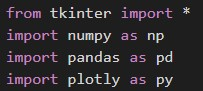
\includegraphics[width=5cm]{Figuras/Bibliotecas.jpg} % leia abaixo
\label{figura:qualquernome}
\end{figure}
 
Na Fig. \ref{figura:qualquernome}, Import das bibliotecas em python
\section{Resultados}

Com a coleta de dados e a demonstração grafica dos mesmos, foi possivel visualizar nitidademente diferenças entre os mesmes iniciais da plataforma, o periodo pre pandemia e o pos pandemia, sendo que os maiores valores são os pos pandemia por uma procura maior por esse tipo de entretenimento virtual.

\begin{figure}[h]
\caption{Tempo em horas}
 
\centering % para centralizarmos a figura
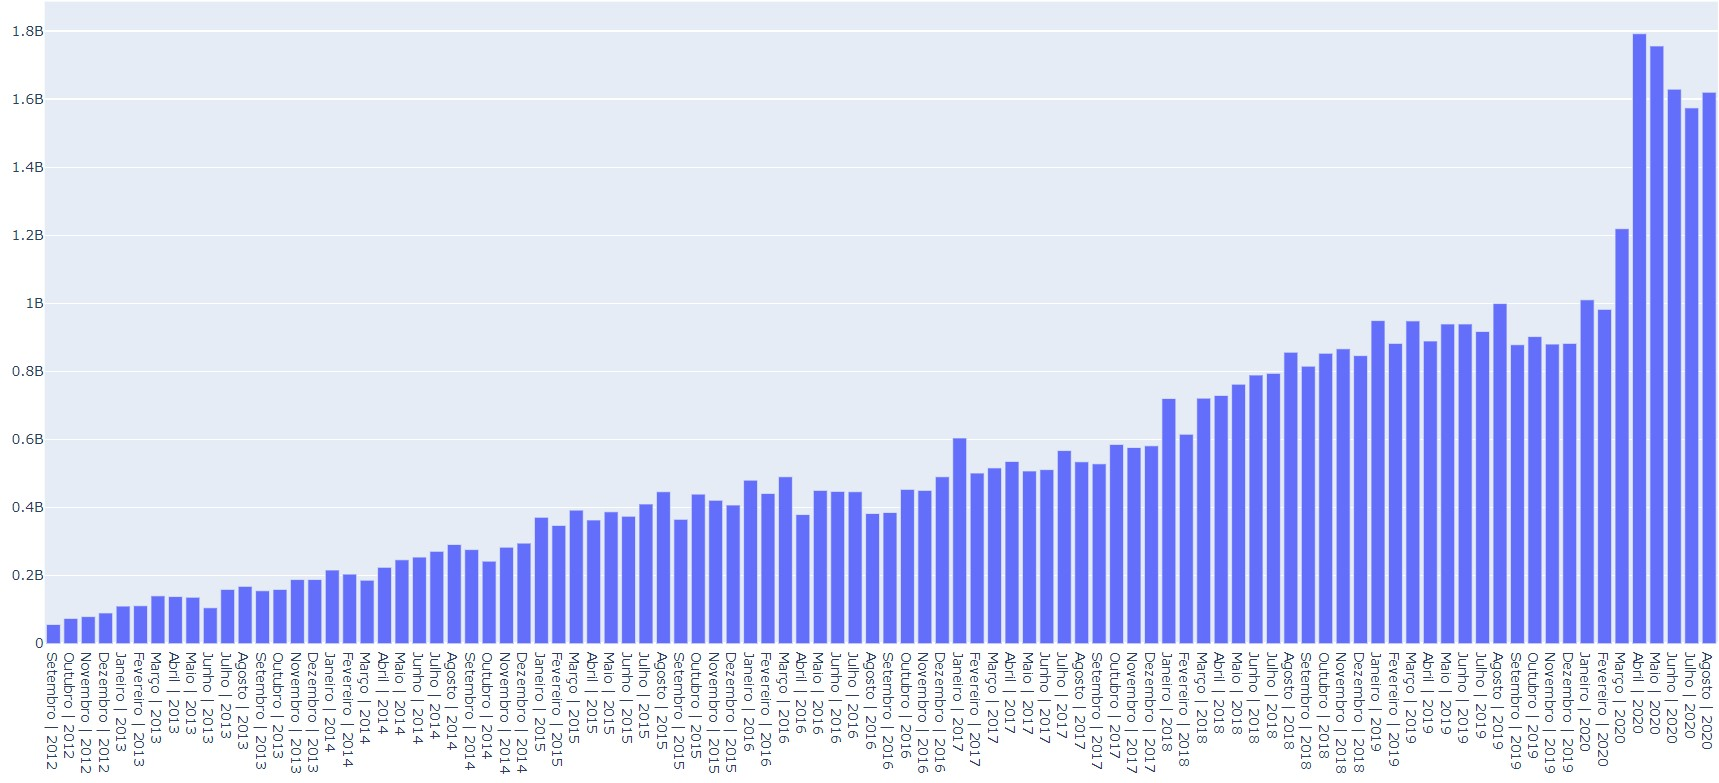
\includegraphics[width=17cm]{Figuras/Tempo_horas.jpg} % leia abaixo
\label{figura:qualquernome}
\end{figure}
Na Fig. \ref{figura:qualquernome}, Grafico em barras do tempo em horas assistido na plataforma

Além disso, é possivel visualizar também a diferença entre quais eram as categorias mais pesquisadas e acessadas no passado e agora, com uma crescente vindo do "just chatting"  desde que se começou a pandemia e alguns sucessos de momento como no caso do "valorant".

\begin{figure}[h]
\caption{Categorias em horas}
 
\centering % para centralizarmos a figura
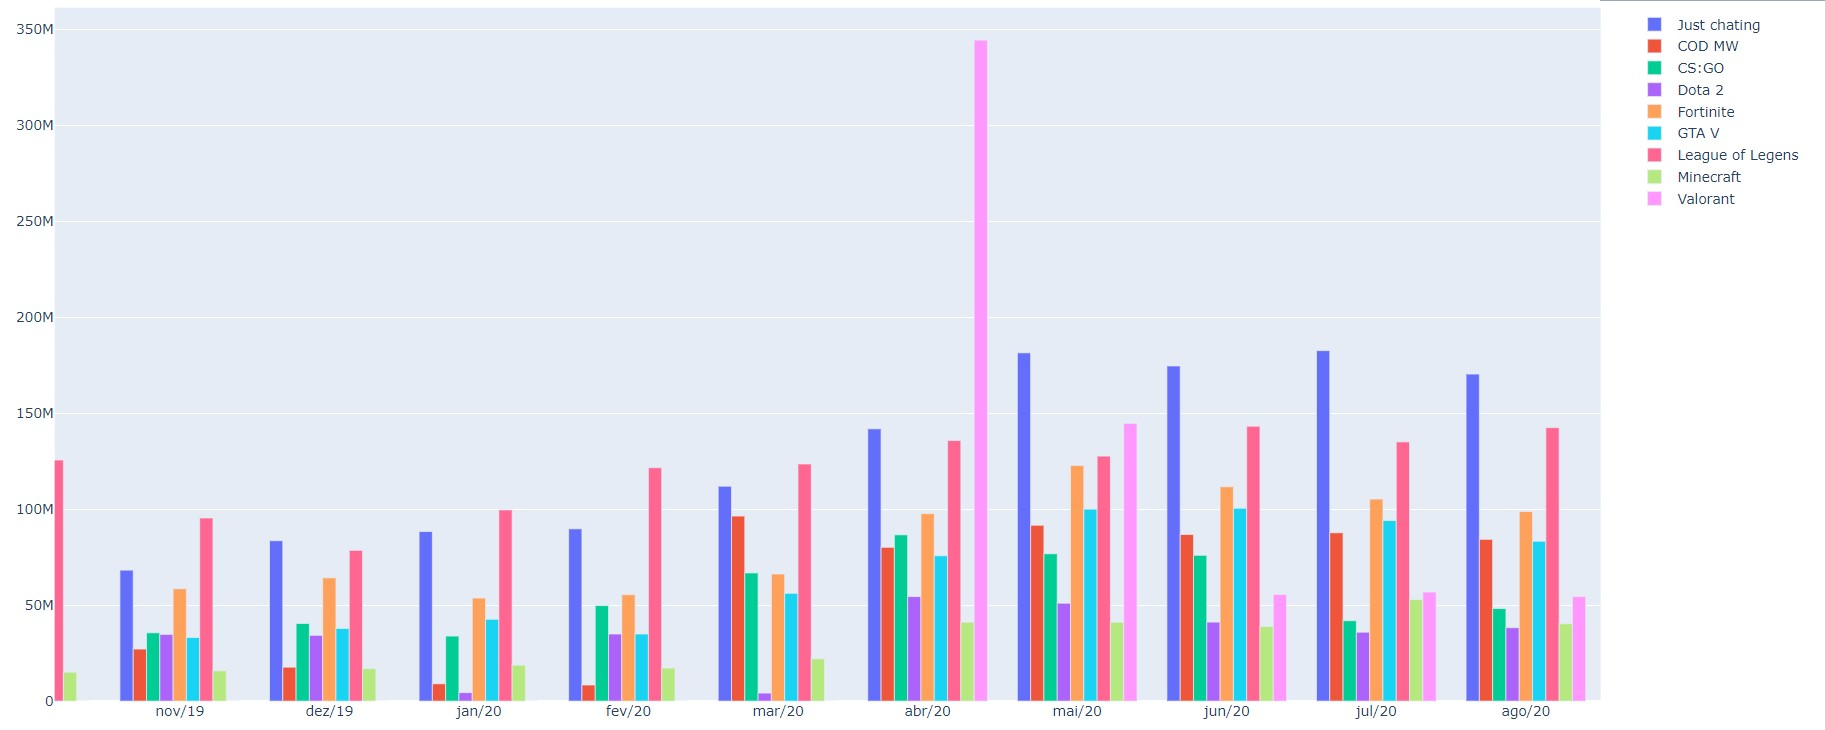
\includegraphics[width=15cm]{Figuras/Categorias_1.jpg} % leia abaixo
\label{figura:qualquernome}
\end{figure}
Na Fig. \ref{figura:qualquernome}, Grafico em barras do tempo em horas assistido das categorias na plataforma


\chapter{Discussão} \label{discussao}

****\textit{Discutir com a orientadora se as seções de resultados e discussão serão mantidas desta forma. Isso vai depender do tipo de pesquisa realizada}. ****

Neste capítulo, são apresentados, interpretados e analisados todos os resultados alcançados no trabalho. A análise deve ser realizada de forma que fique claro se os objetivos específicos foram atendidos. É importante que seja realizada uma comparação com os resultados da literatura, destacando a importância da pesquisa realizada no contexto acadêmico e para o avanço do conhecimento. Ainda, podem ser discutidas, neste capítulo, as limitações e as ameaças a validade do trabalho realizado.


Discutir os resultados\footnote{Para a disciplina de Monografia I, a discussão pode contemplar a descrição de trabalhos futuros, destacando suas proposições, a serem conduzidos durante a disciplina de Monografia II.} obtidos e o trabalho como um todo.


\chapter{Considerações Finais} \label{consideracoes}

Neste capítulo, deve ser explicitado se todos os objetivos descritos na introdução foram atingidos e ressaltar a contribuição do trabalho para o meio acadêmico. O capítulo pode ser subdividido nas seções especificadas a seguir. 



%%====== Section ========%
\section{Conclusão}\label{conclusao}

Em resumo, nesta seção devem ser apresentadas as considerações finais do trabalho. Faça uma recapitulação a respeito de cada um dos objetivos específicos, sintetize os resultados obtidos e conclua se o objetivo principal do trabalho foi alcançado.


%%====== Section ========%
\section{Trabalhos Futuros}\label{trabalhosFuturos}

Apresente propostas de continuidade do seu trabalho.

%%====== Section ========%
\section{Publicações Realizadas}\label{publicacoes}

Caso o trabalho tenha originado publicações é válido acrescentar essa informação, visto que pode creditar ainda mais o estudo. Assim, elas devem ser apresentadas na forma de uma subseção do capítulo conclusão. Por exemplo: 

Os trabalhos seguintes, que foram originados das metodologias propostas, foram aceitos para apresentação em conferências nacionais:

\begin{enumerate}
   \item Autor. Título do Artigo. Cidade: Conferência, Ano.
 \end{enumerate}



%% -------------- Elementos Pós-Textuais -----------------%%
\postextual  
%-------------------------------------------------------------
%---------------------- Apêndices ----------------------------
%-------------------------------------------------------------

\begin{apendicesenv}
\partapendices  % Indica o início dos Apendices

\chapter{Codigo em pyhton}

\begin{figure}[h]
\caption{Tempo em horas}
 
\centering % para centralizarmos a figura
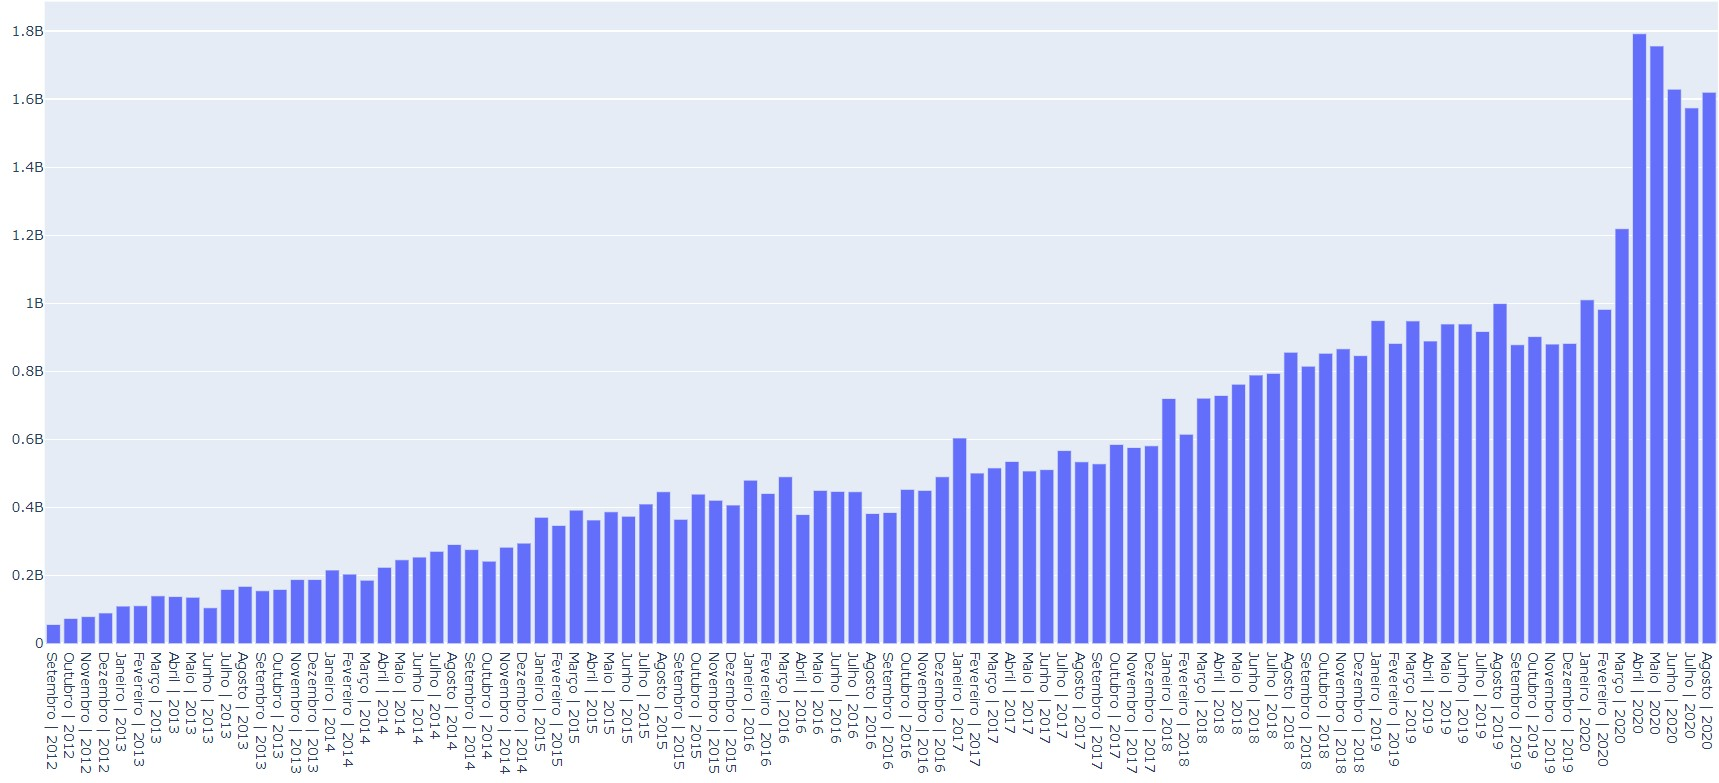
\includegraphics[width=17cm]{Figuras/Tempo_horas.jpg} % leia abaixo
\label{figura:qualquernome}
\end{figure}
Na Fig. \ref{figura:qualquernome}, Grafico em barras do tempo em horas assistido na plataforma
\begin{figure}[h]
\caption{Tempo em horas}
 
\centering % para centralizarmos a figura
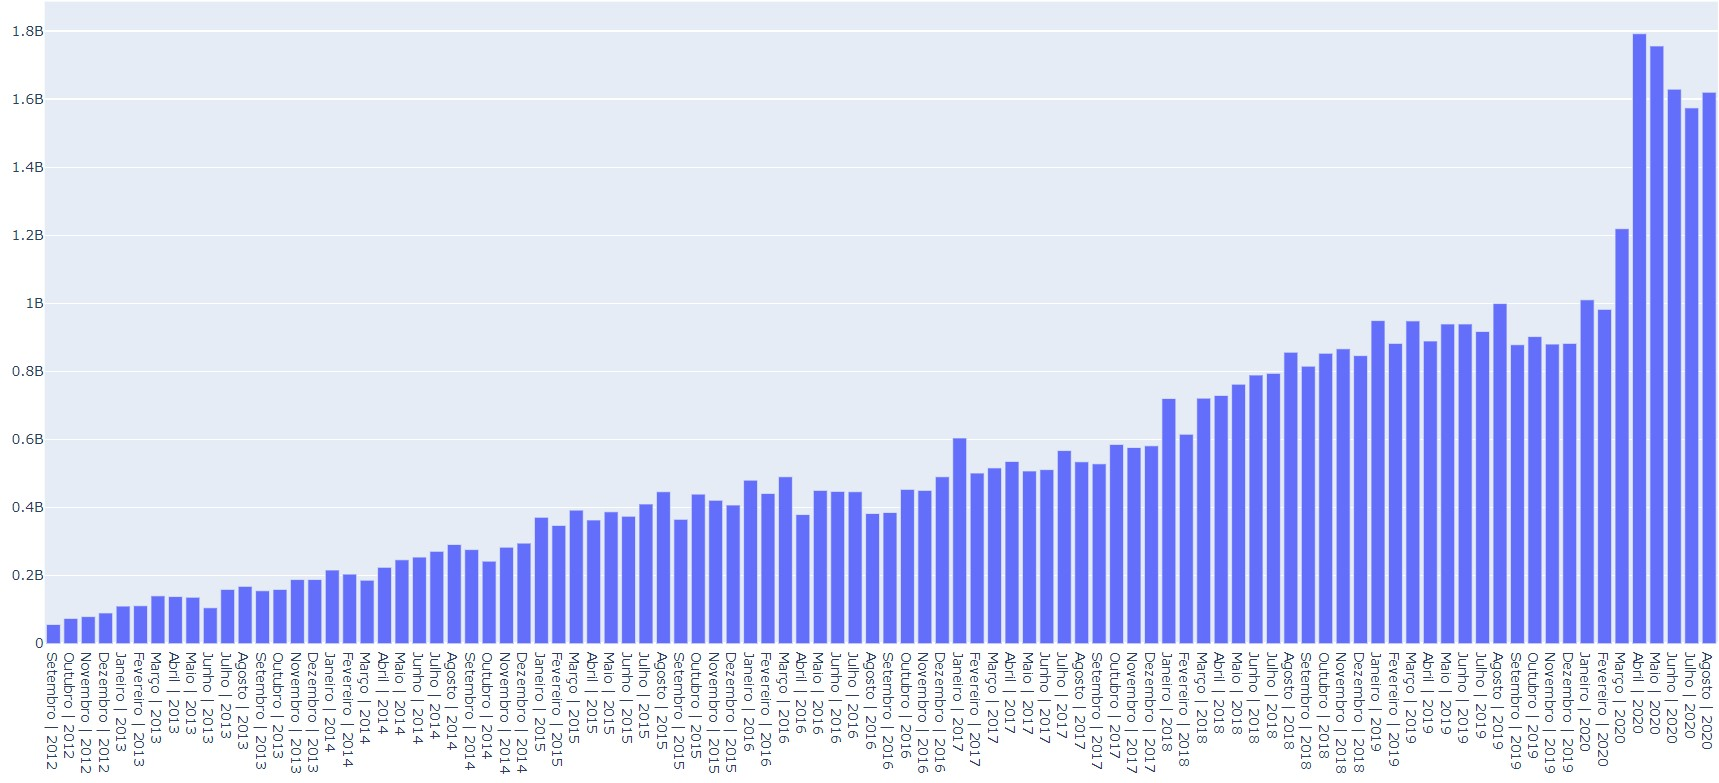
\includegraphics[width=17cm]{Figuras/Tempo_horas.jpg} % leia abaixo
\label{figura:qualquernome}
\end{figure}
Na Fig. \ref{figura:qualquernome}, Grafico em barras do tempo em horas assistido na plataforma
\begin{figure}[h]
\caption{Tempo em horas}
 
\centering % para centralizarmos a figura
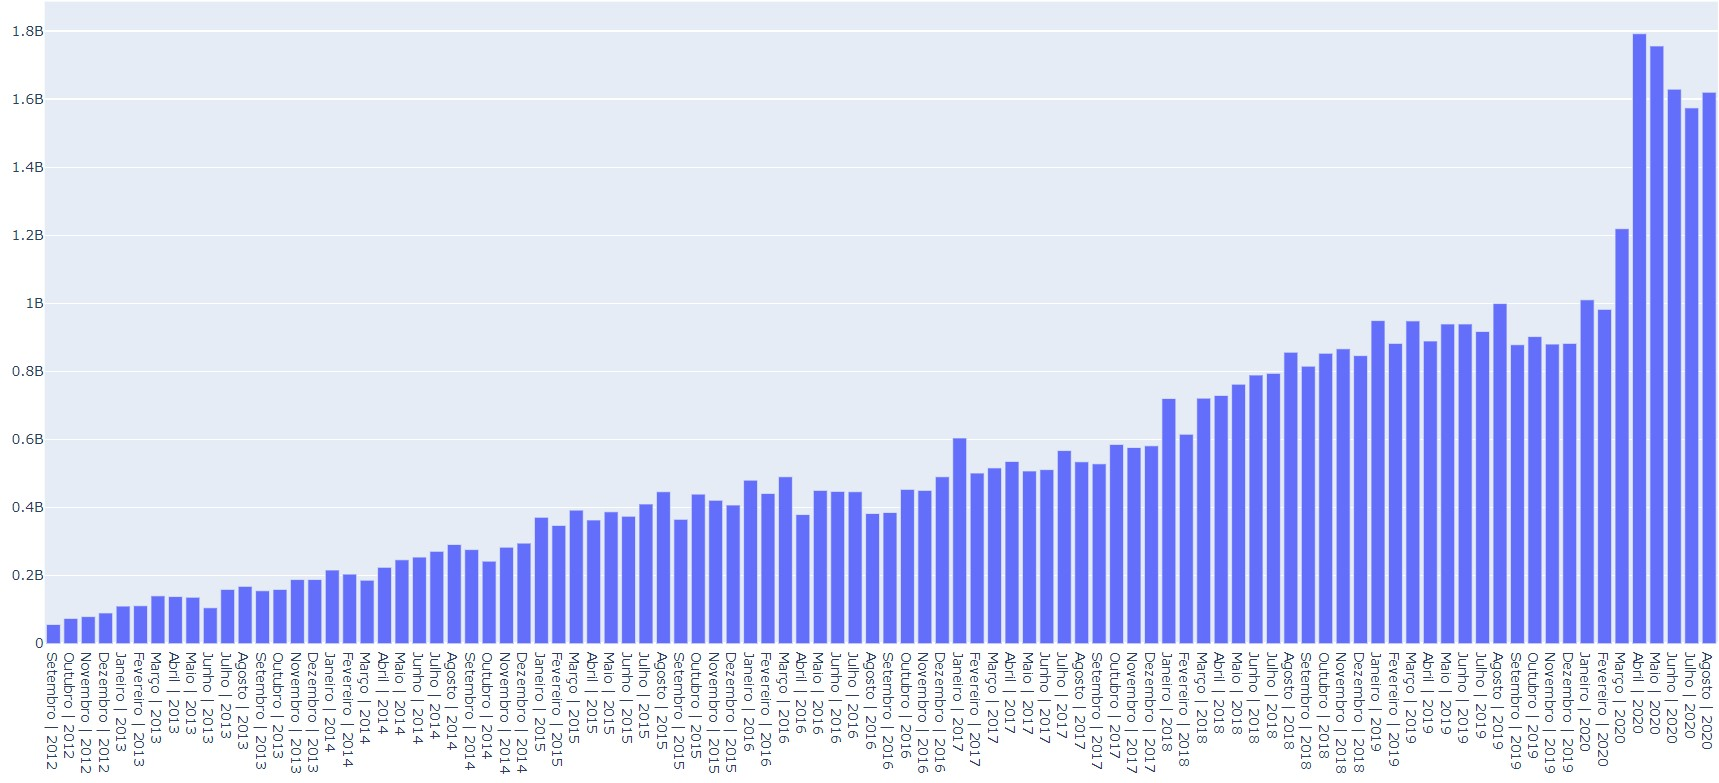
\includegraphics[width=17cm]{Figuras/Tempo_horas.jpg} % leia abaixo
\label{figura:qualquernome}
\end{figure}
Na Fig. \ref{figura:qualquernome}, Grafico em barras do tempo em horas assistido na plataforma
\begin{figure}[h]
\caption{Tempo em horas}
 
\centering % para centralizarmos a figura
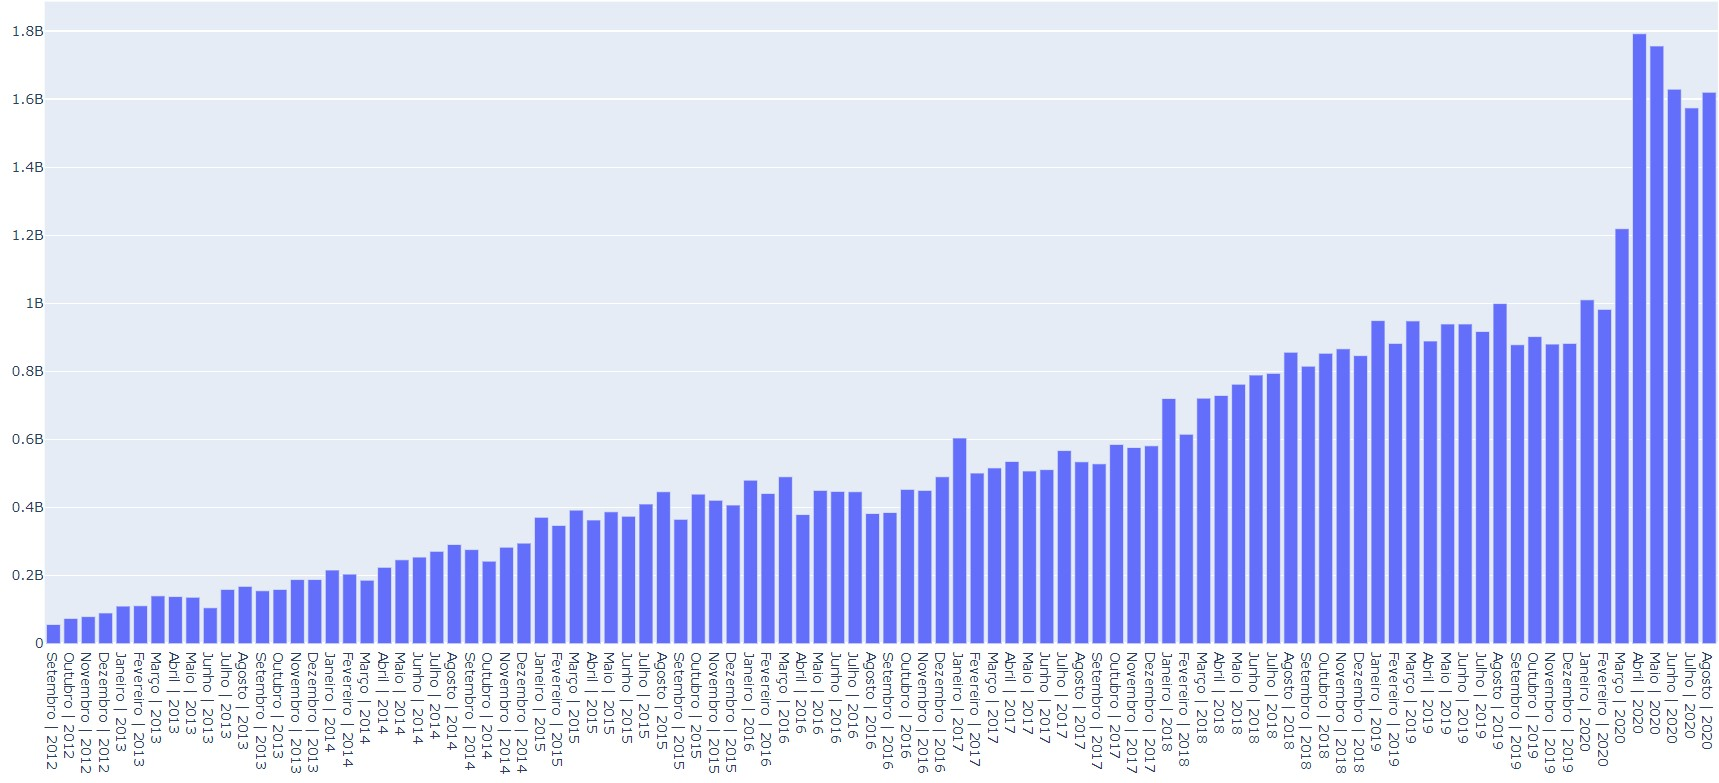
\includegraphics[width=17cm]{Figuras/Tempo_horas.jpg} % leia abaixo
\label{figura:qualquernome}
\end{figure}
Na Fig. \ref{figura:qualquernome}, Grafico em barras do tempo em horas assistido na plataforma

\end{apendicesenv}

%----------------------------------------------------------------
%---------------------- Anexos ----------------------------------
%----------------------------------------------------------------


\phantompart  \printindex  % Indice Remissivo
% ----------------------------------------------------------
\end{document}  % fim do documento
